% =============================================================================
% Working extract -- Results-chapter appendix, all three Qs.
% Content fragment, NOT a standalone compilable document -- meant to be merged
% into the main file's existing \chapter{Appendix} \label{chap:appendix} in
% 20th_1_31_pm_audited.tex (currently an empty placeholder chapter, see its own
% % AUDIT: note listing 7 unresolved \ref calls). This file supplies the
% Results-related ones. Non-Results appendix items (app:hyperparameters,
% app:data-sources, tab:data-env-variables_detail_app -- Data/Methodology
% chapter material) are out of scope here and stay the user's job to fill in
% later, per standing instruction to leave structural/appendix work for last.
%
% Structure: one \section per research question, matching the three working
% results_qN_*.tex files. Each section holds only the appendix material that
% question's Results text actually points to (via \ref) -- built content is
% filled in; not-yet-built content is a short placeholder note, not invented
% numbers.
% =============================================================================

\section{Q1 appendix}
\label{app:results-q1}

\subsection{Full Set4 variable table (EN vs.\ LMM, static/dynamic, stability)}
\label{app:nonlinearity-check}
% Referenced 3x from results_q1_21_08_0754pm.tex (the "one mechanism" paragraphs).
% Source: outputs/spatial_block_kfold/rq2_attribution_nested_set4_gated_all_vif/4survey/fold_{0-4}/,
% built 2026-08-21 -- see that file's own header comment for full provenance.

\begin{table}[!htbp]
\centering
\scriptsize
\setlength{\tabcolsep}{3pt}
\renewcommand{\arraystretch}{1.05}
\begin{tabular}{lrrllll}
\toprule
Variable & EN coef.\ (mean$\pm$SD) & LMM coef.\ (mean$\pm$SD) & Same sign? & Static/Dynamic & Stability verdict & Basis \\
\midrule
CanopyCover & $+1.943\pm0.038$ & $+1.864\pm0.078$ & Yes & Dynamic & Not assessed (leakage check instead) & -- \\
time\_since\_thinning & $-2.139\pm0.216$ & $-1.475\pm0.596$ & Yes & Dynamic & Not assessed & -- \\
time\_since\_thinning\_missing & $-2.995\pm0.182$ & $-1.321\pm0.698$ & Yes & Dynamic & Not assessed & -- \\
recent\_thinning\_5yr & $-0.975\pm0.273$ & $-0.403\pm0.286$ & Yes & Dynamic & Not assessed & -- \\
slope\_degrees & $+0.993\pm0.217$ & $+0.861\pm0.238$ & Yes & Static & \textbf{Stable} & Text-discussed \\
topex & $+0.063\pm0.296$ & $+1.325\pm0.155$ & Yes (Set4 only; flips Set3$\to$Set4) & Static & \textbf{Unstable} & Text-discussed; real local signal (0.09$\to$0.21) \\
tas\_mean & $-0.334\pm0.244$ & $+0.016\pm0.358$ & \textbf{No} & Dynamic & \textbf{Unstable} & Text-discussed; artifact (0.27$\to$0.08) \\
soilgrids\_ph & $+0.123\pm0.186$ & $+0.068\pm0.225$ & Yes (Set4 only) & Static & \textbf{Unstable} & Text-discussed; artifact (0.27$\to$0.05) \\
chelsa\_bio12\_precip\_mm & $-0.620\pm0.505$ & $-1.417\pm0.618$ & Yes & Static & \textbf{Stable} (EN/LMM agree) & Text-discussed; local-signal retention ($-0.298\to-0.0996$, 33\%) is close to the confirmed-artifact tas\_mean's (32\%) -- stability here rests on EN/LMM agreement itself, not a clearly demonstrated surviving local signal like topex's (267\%) \\
ceh\_twi & $-0.038\pm0.174$ & $+0.053\pm0.047$ & \textbf{No} & Static & \textbf{Unstable (new)} & Found this session; artifact ($-0.10\to0.01$) \\
gwa\_weibull\_a\_50m & $-0.579\pm0.609$ & $+0.342\pm0.066$ & \textbf{No} & Static & \textbf{Unstable (new)} & Found this session; real local signal ($-0.34\to-0.14$) \\
local\_relief\_500m & $+0.163\pm0.110$ & $-0.122\pm0.254$ & \textbf{No} & Static & \textbf{Unstable (new)} & Found this session; artifact ($-0.15\to0.00$) \\
gwa\_weibull\_k\_50m & $-0.135\pm0.196$ & $-0.359\pm0.249$ & Yes & Static & Not assessed & -- \\
gwa\_weibull\_a\_10m & $-0.082\pm0.094$ & $-0.111\pm0.056$ & Yes & Static & Not assessed & -- \\
gwa\_wind\_speed\_10m & $-0.121\pm0.074$ & $-0.108\pm0.068$ & Yes & Static & Not assessed & -- \\
eastness & $+0.471\pm0.087$ & $+0.326\pm0.019$ & Yes & Static & Not assessed & -- \\
dist\_to\_scpt\_boundary & $-0.299\pm0.103$ & $-0.146\pm0.071$ & Yes & Static & Not assessed & -- \\
dist\_to\_road & $-1.332\pm0.171$ & $-1.216\pm0.130$ & Yes & Static (vintage uncertain) & Not assessed (own role in leakage check) & -- \\
whcl & $-0.594\pm0.228$ & $-0.459\pm0.400$ & Yes & Static (not verified) & Not assessed & -- \\
\bottomrule
\end{tabular}
\caption{\small{Set4 (4-survey), all 19 variables: Elastic Net vs.\ mixed-effects (LMM) coefficients (mean $\pm$ SD, 5 folds), whether they agree in sign, static/dynamic classification, and stability verdict. ``Same sign?'' is a simplified same-fold-set check, not identical to the fuller stable/unstable definition used in-text (which also considers cross-set consistency and coefficient-vs-SD magnitude) -- topex and soilgrids\_ph pass this simplified sign check in Set4 alone but are still classed unstable by the fuller definition. Rows marked ``Not assessed'' were never individually checked for stability in the main text; their EN/LMM sign agreement here is offered as a first-pass screen, not a final verdict.}}
\label{tab:q1-set4-full-variable-table}
\end{table}

\begin{figure}[!htbp]
\centering
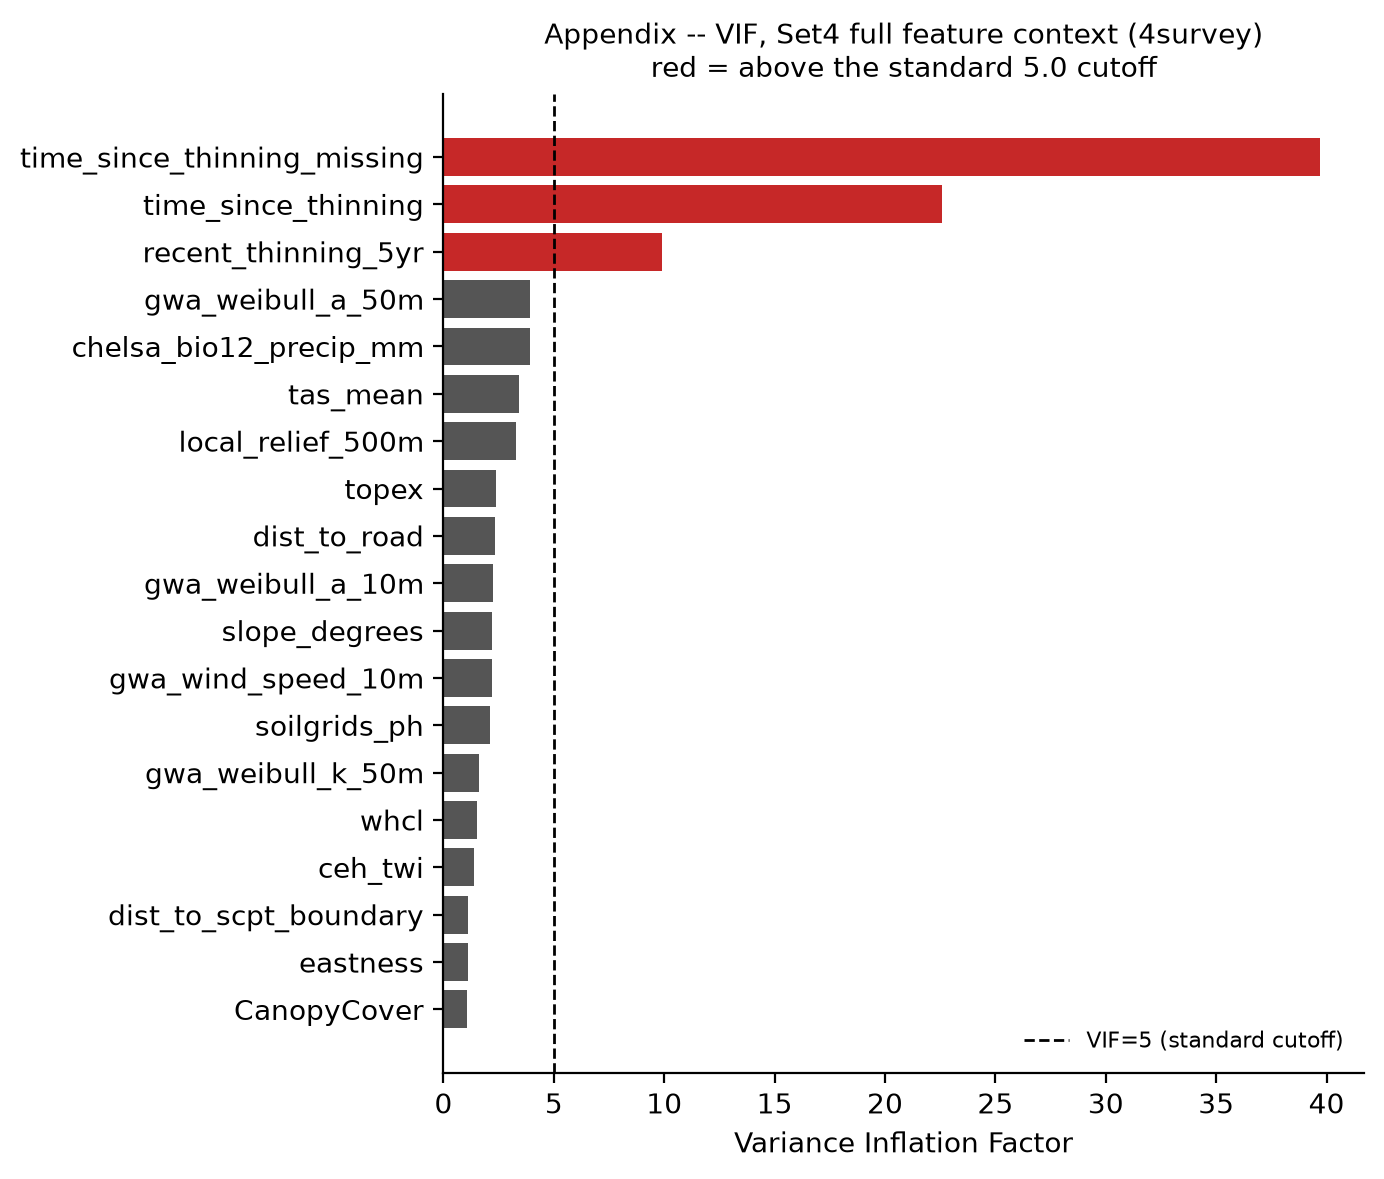
\includegraphics[width=0.6\textwidth]{figures/fig_results/q1_selected_appendix_vif.png}
\caption{\small{Variance inflation factor (VIF) for all 19 Set4 columns (4-survey), computed live via \texttt{compute\_vif\_table()}. Only the 3 thinning/management columns exceed the standard VIF=5 cutoff (expected -- \texttt{time\_since\_thinning} and its missingness flag are closely related by construction); all abiotic (terrain/climate/soil) variables discussed in the main text, including the 6 unstable ones, have VIF well under 5, ruling out multicollinearity as their cause.}}
\label{fig:q1-appendix-vif}
\end{figure}

\subsection{Category-level ablation (soil / climate / terrain)}
\label{app:category-ablation}
% AUDIT: placeholder -- referenced once from results_q1 ("full ablation in Appendix~\ref{app:category-ablation}"),
% not yet built here. The headline numbers already quoted in the main text (soil +0.022 R2, climate -0.056 R2,
% Set4 category refit) need their source table/run reproduced and placed here -- not yet done this session.

\section{Q2 appendix}
\label{app:results-q2}

\subsection{Flagged-plot split diagnostics}
\label{app:flagged-plot-split}
% AUDIT: placeholder -- referenced once from results_q2 (fixed-k curve-fitting artifact vs.\ genuine rapid growth
% in the 266 Tukey-flagged plots). Source diagnostics exist in TEMP_results_attribution/ per earlier session work
% (see handover docs) but have not been transcribed into this appendix yet.

\subsection{Category-level Moran's I diagnostics (with terrain bandwidth-artifact adjustment)}
\label{app:results-q2-category-morans-i}
% AUDIT: placeholder -- results_q2 currently points this content at the generic \ref{chap:appendix} rather than
% a specific label; once this subsection is filled in, update that in-text ref to
% \ref{app:results-q2-category-morans-i} instead.

\section{Q3 appendix}
\label{app:results-q3}

\subsection{Full 6-survey table}
\label{app:results-q3-6survey}
% Moved out of the main Table~\ref{tab:results-q3} 2026-08-23 for clarity, since 6-survey is
% not this chapter's main analysis surface (see that table's caption). PINN/PINN-k rows show
% -- : the corrected-forward-pass work this chapter reports (environment sweep, lambda
% ablation, hyperparameter checks -- see temp_results_pinn/RESULTS_TABLE.md) was all done on
% 4-survey only; 6-survey was never rerun with the corrected architecture, and the pre-fix
% 6-survey numbers are not valid evidence for the corrected model (same reasoning as the
% pre-fix PINN runs excluded from the main table).

\begin{table}[!htbp]
\centering
\scriptsize
\setlength{\tabcolsep}{4pt}
\renewcommand{\arraystretch}{1.2}
\begin{tabular}{lrrr}
\toprule
Model & RMSE${\downarrow}$ & MAE${\downarrow}$ & $R^2{\uparrow}$ \\
\midrule
Linear & $4.877{\pm}0.643$ & $3.619{\pm}0.426$ & $0.509{\pm}0.067$ \\
RF & $4.062{\pm}0.249$ & $3.010{\pm}0.185$ & $0.656{\pm}0.046$ \\
XGBoost (tuned) & $\mathbf{3.656{\pm}0.232}$ & $\mathbf{2.669{\pm}0.183}$ & $\mathbf{0.722{\pm}0.031}$ \\
DNN & $3.903{\pm}0.316$ & $2.867{\pm}0.275$ & $0.684{\pm}0.031$ \\
PINN & -- & -- & -- \\
PINN-$k$ & -- & -- & -- \\
\bottomrule
\end{tabular}
\caption{\small{Model comparison for top-height prediction, 6-survey, Set3,
spatial\_block\_kfold, per-fold mean $\pm$ SD across five folds. n=82{,}614 row-years
(13{,}769 plots). Referenced from the main text's DNN-vs.-XGBoost fold-count and
compartment-subsampling discussion. PINN/PINN-$k$ were not rerun with the corrected
forward pass on this cohort (--); see main-text Table~\ref{tab:results-q3}'s caption.}}
\label{tab:results-q3-6survey}
\end{table}

\subsection{Pre-fix PINN runs (uncorrected baseline, for comparison)}
\label{app:results-q3-prefix-pinn}
% AUDIT: placeholder -- results_q3 currently points this content at the generic \ref{chap:appendix} rather than
% a specific label; once this subsection is filled in, update that in-text ref to
% \ref{app:results-q3-prefix-pinn} instead.
